\documentclass[a4paper,12pt]{article}

\usepackage[utf8]{inputenc}
\usepackage[spanish]{babel}
\usepackage{amsmath, amssymb}
\usepackage{graphicx}
\usepackage{float}
\usepackage{booktabs}
\usepackage{xcolor}
\usepackage{listings}
\usepackage{caption}
\usepackage{fancyhdr}
\usepackage{hyperref}
\usepackage{tikz}

\hypersetup{
    colorlinks=true,
    linkcolor=blue,
    urlcolor=blue,
    pdftitle={Práctica 2 - ESP32},
}

% ---------- PREÁMBULO: arreglar comillas en listings (Thonny style) ----------
\usepackage[utf8]{inputenc}   % si no está ya
\usepackage[T1]{fontenc}      % mejor soporte de tipografías para PDFs
\usepackage{textcomp}         % símbolos de texto adicionales
\usepackage{upquote}          % comillas ' y " tipo ASCII en verbatim/listings

% Si usas babel con español, desactiva el shorthand de la comilla doble
\usepackage[spanish]{babel}
\shorthandoff{"}  % <<< evita que " sea un caracter activo (causa comillas invisibles)

% Colores inspirados en Thonny
\usepackage{xcolor}
\definecolor{thonnyKeyword}{rgb}{0.0,0.2,0.8}
\definecolor{thonnyComment}{rgb}{0.0,0.5,0.0}
\definecolor{thonnyString}{rgb}{0.7,0.12,0.12}
\definecolor{thonnyBackground}{rgb}{1.0,1.0,1.0}
\definecolor{thonnyBuiltin}{rgb}{0.5,0.0,0.5}
\definecolor{thonnyNumber}{rgb}{0.35,0.35,0.35}

% Declaración de lenguaje MicroPython (basado en Python)
\usepackage{listings}
\lstdefinelanguage{MicroPython}{
    morekeywords={
        False, True, None, and, as, assert, async, await, break, class, continue,
        def, del, elif, else, except, finally, for, from, global, if, import,
        in, is, lambda, nonlocal, not, or, pass, raise, return, try, while, with, yield
    },
    morekeywords=[2]{print,open,range,len,abs,int,float,str,dict,list,set,tuple},
    morekeywords=[3]{machine,network,time,urequests,utime,gc,Pin,ADC,PWM,UART,RTC,ESP32},
    sensitive=true,
    morecomment=[l]{\#},
    morestring=[b]",
    morestring=[b]',
}

% Configuración de listings con estilo Thonny (y upquote activo)
\lstset{
    language=MicroPython,
    backgroundcolor=\color{thonnyBackground},
    keywordstyle=\color{thonnyKeyword}\bfseries,
    keywordstyle=[2]\color{thonnyBuiltin},
    keywordstyle=[3]\color{thonnyKeyword!60!black},
    commentstyle=\color{thonnyComment}\itshape,
    stringstyle=\color{thonnyString},
    numberstyle=\tiny\color{thonnyNumber},
    basicstyle=\ttfamily\small,
    numbers=left,
    numbersep=6pt,
    frame=single,
    framerule=0.4pt,
    breaklines=true,
    breakatwhitespace=true,
    showstringspaces=false,
    tabsize=2,
    captionpos=b,
    columns=flexible,
    upquote=true     % importante para mostrar comillas rectas correctamente
}

\title{Práctica N°2: Inicializacion en ESP32 manejo de ADC y GPIO}
\date{}

\begin{document}
\maketitle
\tableofcontents
\newpage

\section{Objetivos}

\subsection{Objetivo general}
Desarrollar y documentar, paso a paso, una práctica didáctica para programar un ESP32 WROOM-32 con MicroPython usando el entorno Thonny. La práctica cubrirá desde la configuración y carga de firmware hasta la implementación, prueba y verificación de programas básicos de entrada/salida digital, lectura analógica y sensores DHT, fomentando buenas prácticas de cableado, protección (resistencias) y manejo de errores.

\subsection{Objetivos específicos}
\begin{itemize}
  \item \textbf{Parpadeo LED (blink\_pin5.py):} Implementar un programa que haga parpadear un LED conectado a GPIO5 con periodo aproximado de 1\,s. 
  
  \item \textbf{Control por pulsador con pull-up interno (led\_button\_gpio16.py):} Integrar un pulsador conectado a GPIO16 usando la resistencia de pull-up interna del ESP32 y gestionar el rebote por software (debounce). El pulsador deberá encender el LED al presionarse y apagarlo al soltarse. 
  
  \item \textbf{Lectura analógica de potenciómetro (adc\_pot\_esp32.py):} Configurar un ADC en GPIO34 (ADC1\_CH6) con atenuación adecuada (ATTN\_11DB) y resolución de 12 bits; leer y escalar a voltaje real (0--3.3\,V). 
  
  \item \textbf{Sensor DHT11 (dht11\_gpio4.py):} Conectar y leer un sensor DHT11 en GPIO4, implementando manejo de excepciones para lecturas erróneas y periodos de muestreo apropiados.
  
  
\end{itemize}

\section{Configuración inicial del entorno y carga de firmware MicroPython}

Antes de ejecutar cualquier programa en el ESP32, es necesario instalar el firmware de \textbf{MicroPython} dentro del microcontrolador. A continuación se describe el procedimiento completo usando el entorno \textbf{Thonny IDE}, disponible para Windows, Linux y macOS. En esta guía se empleará la versión para Windows.

\subsection{Requisitos previos}
\begin{itemize}
  \item Computadora con sistema operativo Windows 10 o superior.
  \item IDE Thonny instalado (\url{https://thonny.org}).
  \item Módulo ESP32 WROOM-32 o tarjeta de desarrollo equivalente.
  \item Cable USB tipo micro (datos, no sólo carga).
  \item Firmware oficial de MicroPython para ESP32 (\texttt{.bin}), descargable desde:
  \url{https://micropython.org/download/esp32/}.
\end{itemize}

\subsection{Conexión del ESP32 al PC}
Conecta el ESP32 a la computadora mediante el cable USB.  
El sistema operativo debe reconocer el dispositivo como un puerto serial (por ejemplo, \texttt{COM3} o similar).

Si el puerto no aparece, puede ser necesario instalar los controladores USB del chip CP2102 o CH340, dependiendo del modelo del módulo ESP32.

\subsection{Configuración inicial en Thonny}
Abre Thonny y selecciona el intérprete adecuado:

\begin{enumerate}
  \item Ve al menú \texttt{Herramientas → Opciones → Intérprete}.
  \item En el campo \texttt{Ejecutar en}, selecciona: \textbf{MicroPython (ESP32)}.
  \item En el campo \texttt{Puerto}, elige el puerto COM correspondiente a tu placa.
\end{enumerate}

\begin{figure}[H]
  \centering
  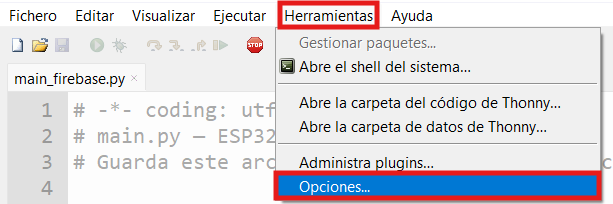
\includegraphics[width=0.8\textwidth]{Thonny/Interprete.png}
  \caption{Configuración del intérprete MicroPython (ESP32) en Thonny.}
\end{figure}

\begin{figure}[H]
  \centering
  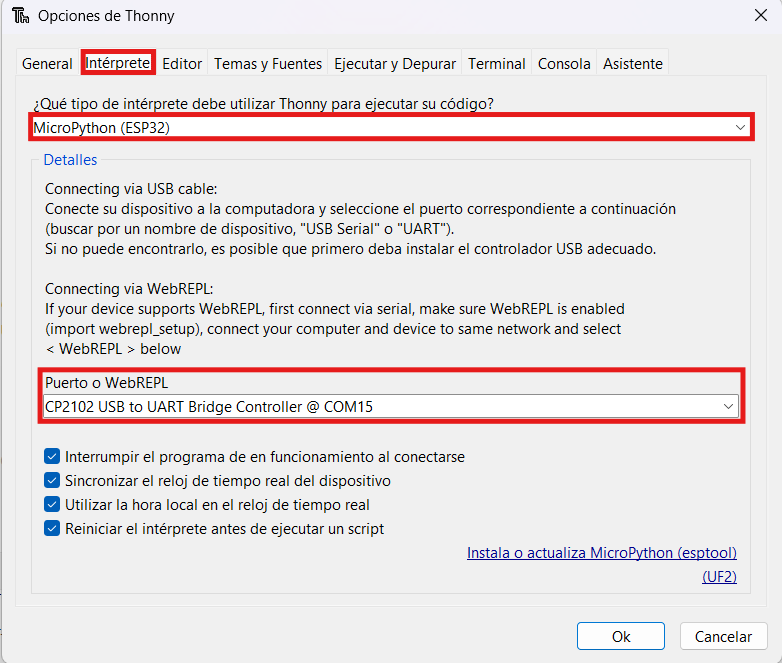
\includegraphics[width=0.8\textwidth]{Thonny/Interprete_2.png}
  \caption{Configuración del intérprete MicroPython (ESP32) en Thonny.}
\end{figure}

\subsection{Instalación del firmware MicroPython (flasheo)}
Si el ESP32 no tiene MicroPython instalado o se desea actualizarlo, Thonny permite flashear el firmware directamente:

\begin{enumerate}
  \item En el mismo cuadro de diálogo de \texttt{Opciones → Intérprete}, haz clic en el botón \textbf{Instalar o actualizar firmware}.
  \item Selecciona el puerto correcto (\texttt{COMx}).
  \item Pulsa en \textbf{Buscar firmware en micropython.org}. Thonny descargará automáticamente la versión estable más reciente.
  \item Marca la opción \textbf{Borrar completamente el chip antes de instalar}.
  \item Finalmente, presiona \textbf{Instalar}.
\end{enumerate}

\begin{figure}[H]
  \centering
  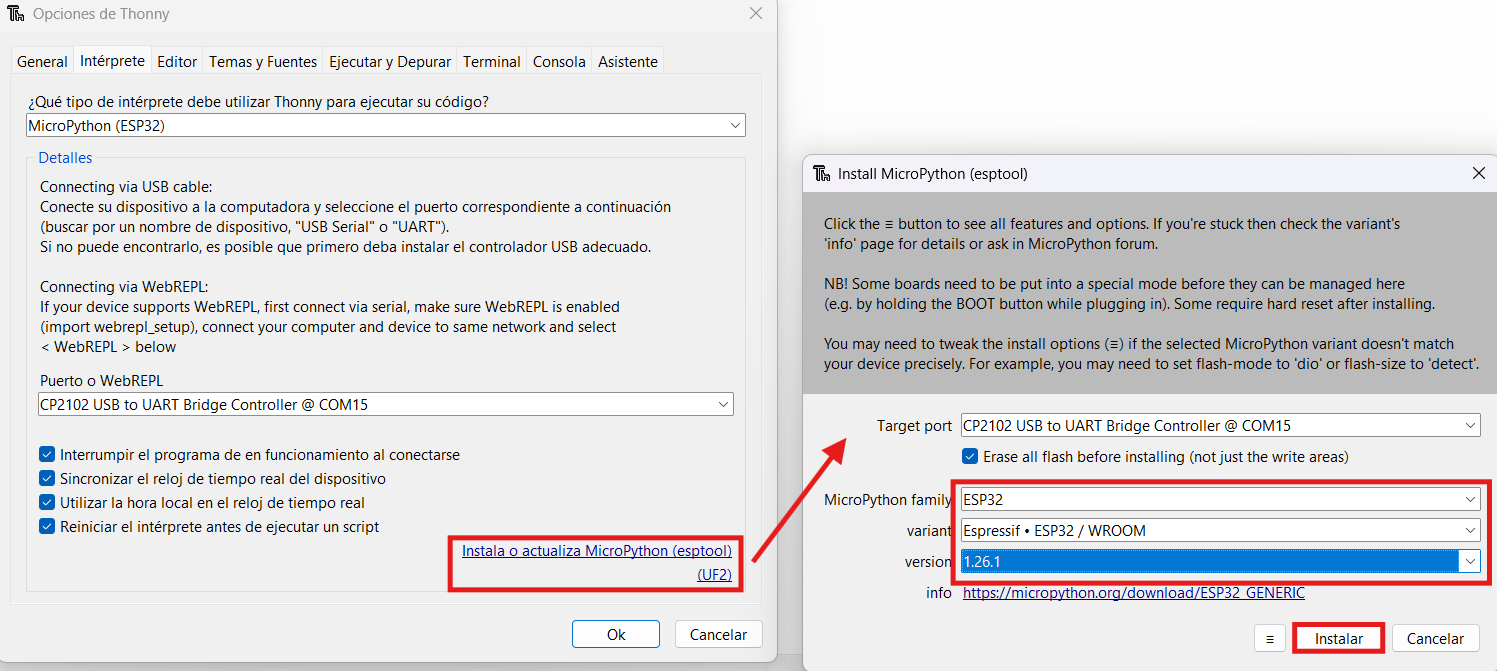
\includegraphics[width=0.8\textwidth]{Thonny/firmware.png}
  \caption{Ventana de instalación o actualización de firmware MicroPython en Thonny.}
\end{figure}

Durante el proceso, se mostrará el progreso en la barra inferior. Este paso puede tardar entre 30 y 60 segundos.  
Al finalizar, Thonny mostrará el mensaje \texttt{Firmware installation successful}.

\begin{figure}[H]
  \centering
  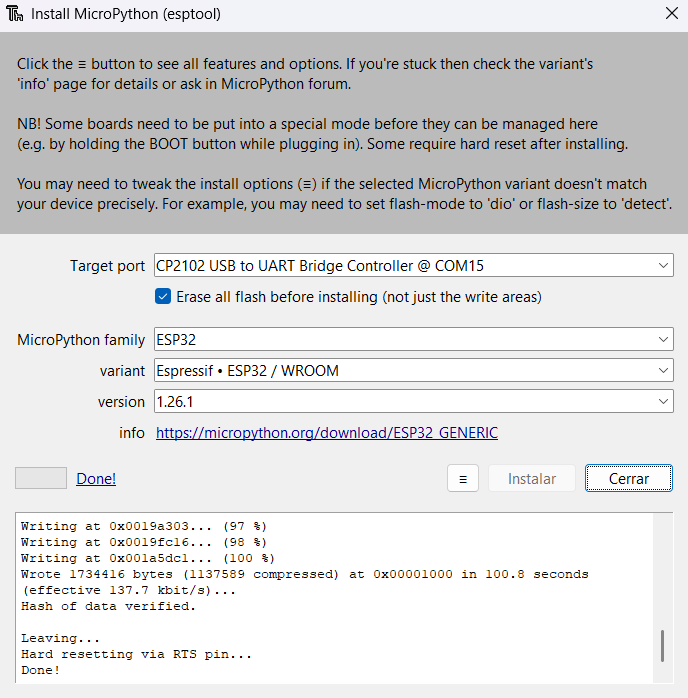
\includegraphics[width=0.7\textwidth]{Thonny/firmware_3.png}
  \caption{Proceso de flasheo del firmware MicroPython en el ESP32 completado.}
\end{figure}

\subsection{Verificación de instalación}
Una vez cargado el firmware:

\begin{enumerate}
  \item Cierra y vuelve a abrir Thonny.
  \item Asegúrate de que el intérprete seleccionado sea nuevamente \textbf{MicroPython (ESP32)}.
  \item En la consola inferior aparecerá un mensaje similar a:
\begin{verbatim}
MicroPython v1.22.0 on 2025-01-15; ESP32 module with ESP32
Type "help()" for more information.
>>>
\end{verbatim}
\end{enumerate}

\begin{figure}[H]
  \centering
  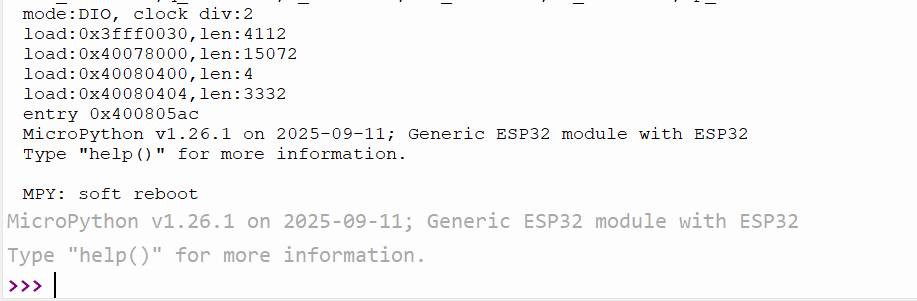
\includegraphics[width=0.7\textwidth]{Thonny/RELP.png}
  \caption{Consola REPL de MicroPython lista para recibir comandos.}
\end{figure}

\section{Explicación del código}

En esta sección se analiza el funcionamiento de cada uno de los programas desarrollados en MicroPython para el ESP32. Más que una simple descripción, el propósito es comprender la lógica detrás de cada bloque de código, reconociendo la relación entre el hardware y las instrucciones que lo controlan.

\newpage

\subsection{Parpadeo simple del LED en GPIO5}

\begin{lstlisting}[language=Python, caption={Parpadeo simple del LED en GPIO5}]
# blink_pin5.py
# MicroPython para ESP32 WROOM-32
# Conecta un LED (con resistencia) al pin GPIO5 (GND compartido)

import machine
import time

print("Prueba ESP32 - parpadeo en GPIO5")

led = machine.Pin(5, machine.Pin.OUT)

while True:
    led.value(not led.value())  # toggle
    time.sleep(1)
\end{lstlisting}

El código comienza importando las librerías \texttt{machine} y \texttt{time}, esenciales para acceder al hardware y controlar retardos. La creación del objeto \texttt{Pin(5, Pin.OUT)} configura el GPIO5 como salida digital, donde se conecta el LED.  
Dentro del bucle infinito, el estado del pin se invierte en cada iteración, generando un parpadeo continuo. El retardo de un segundo, introducido por \texttt{time.sleep(1)}, hace visible la oscilación. Este ejemplo representa el punto de partida en el control digital del ESP32, donde cada instrucción tiene un reflejo inmediato en el hardware.

\subsection{Control del LED mediante pulsador (GPIO16)}

\begin{lstlisting}[language=Python, caption={Manejo del LED con un pulsador usando PULL\_UP interno}]
# led_button_gpio16.py
from machine import Pin
import time

led = Pin(5, Pin.OUT)
button = Pin(16, Pin.IN, Pin.PULL_UP)

DEBOUNCE_MS = 50
last_state = button.value()
last_time = time.ticks_ms()

while True:
    state = button.value()
    if state != last_state:
        t = time.ticks_ms()
        if time.ticks_diff(t, last_time) > DEBOUNCE_MS:
            last_state = state
            last_time = t
            if state == 0:
                led.on()
            else:
                led.off()
    time.sleep_ms(10)
\end{lstlisting}

Aquí el programa introduce la interacción entre entrada y salida. El LED conectado al GPIO5 se controla mediante un pulsador en el GPIO16, el cual utiliza una resistencia \textit{pull-up} interna.  
El código aplica una técnica de \textit{antirrebote} por software, verificando que el tiempo entre cambios de estado supere un umbral definido por \texttt{DEBOUNCE\_MS}. Así se evita que los rebotes eléctricos del pulsador generen falsas detecciones.  
El resultado es una respuesta estable: el LED se enciende solo cuando el botón se mantiene presionado. Este ejemplo muestra la transición desde la lógica puramente digital hacia un control más robusto y realista, incorporando consideraciones físicas del hardware.

\subsection{Lectura analógica de un potenciómetro}

\begin{lstlisting}[language=Python, caption={Lectura analógica desde GPIO34}]
# adc_pot_esp32.py
from machine import Pin, ADC
import time

pot = ADC(Pin(34))
pot.atten(ADC.ATTN_11DB)
pot.width(ADC.WIDTH_12BIT)

while True:
    raw = pot.read()
    volts = raw / 4095 * 3.3
    print("ADC raw:", raw, "-> {:.2f} V".format(volts))
    time.sleep(0.5)
\end{lstlisting}

El uso del módulo \texttt{ADC} introduce la lectura analógica en el ESP32. Al conectar un potenciómetro al pin GPIO34, el programa mide valores de 0 a 4095, correspondientes al rango de tensión configurado mediante \texttt{ADC.ATTN\_11DB}.  
El cálculo de voltaje convierte los datos en una escala física más comprensible, mostrando en consola el valor aproximado en voltios. Este ejemplo marca el paso hacia una lectura continua y cuantitativa, donde la información del entorno se transforma en datos numéricos útiles.

    



\section{Carga y ejecución de programas en el ESP32 con Thonny}

Una vez instalado el firmware de MicroPython y verificado el funcionamiento básico del intérprete, se pueden crear y ejecutar programas directamente desde el entorno Thonny. Esta sección muestra el procedimiento completo para subir y probar el primer programa: el parpadeo del LED conectado al pin GPIO5.

\subsection{Creación del archivo fuente}
Abre Thonny y selecciona la pestaña de un nuevo archivo mediante el menú \texttt{Archivo → Nuevo}.  
Escribe el siguiente código, correspondiente al programa de parpadeo simple:

\begin{lstlisting}[language=Python, caption={blink\_pin5.py -- Parpadeo del LED en GPIO5}, label={lst:blink}]
# blink_pin5.py
# MicroPython para ESP32 WROOM-32
# Conecta un LED (con resistencia) al pin GPIO5 (GND compartido)

import machine
import time

print("Prueba ESP32 - parpadeo en GPIO5")

led = machine.Pin(5, machine.Pin.OUT)

while True:
    led.value(not led.value())  # toggle
    time.sleep(1)
\end{lstlisting}



\subsection{Guardar el archivo en el ESP32}
Al intentar guardar el programa, Thonny mostrará una ventana preguntando dónde hacerlo.  
Selecciona la opción \textbf{Guardar en el dispositivo MicroPython}.

\begin{figure}[H]
  \centering
  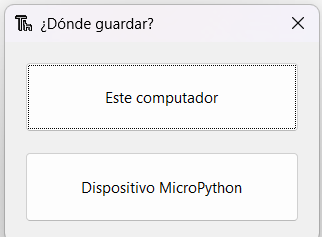
\includegraphics[width=0.8\textwidth]{MicroPython/ubicacion.png}
  \caption{Guardado del archivo directamente en el sistema de archivos del ESP32.}
\end{figure}

Se recomienda usar nombres cortos y sin espacios, por ejemplo:  
\texttt{blink.py}, \texttt{pot.py}, \texttt{dht.py}, etc.  
Los scripts almacenados en la memoria del ESP32 pueden ejecutarse incluso sin conexión al PC (dependiendo de cómo se configuren).

\subsection{Ejecución del programa}
Para ejecutar el código, presiona el botón \textbf{Ejecutar} (ícono de triángulo verde) o usa el atajo \texttt{F5}.  
En la consola inferior se mostrará el texto del programa y el LED conectado al pin GPIO5 comenzará a parpadear con una frecuencia aproximada de 1\,Hz.

\begin{figure}[H]
  \centering
  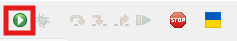
\includegraphics[width=0.8\textwidth]{MicroPython/play.png}
  \caption{Ejecución del programa de parpadeo desde Thonny.}
\end{figure}

\subsection{Detención del programa}
Para detener la ejecución, presiona el botón \textbf{Detener/Interrumpir} (ícono cuadrado rojo) en la barra superior de Thonny.  
Esto envía una interrupción al bucle principal del programa (equivalente a \texttt{Ctrl+C} en la consola REPL).

\begin{figure}[H]
  \centering
  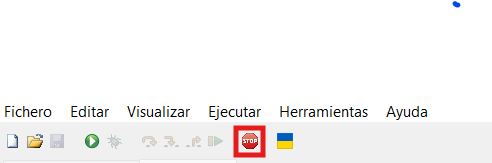
\includegraphics[width=0.7\textwidth]{MicroPython/stop.png}
  \caption{Detención manual del programa en ejecución.}
\end{figure}

\subsection{Ejecución automática al encender el ESP32}
MicroPython permite ejecutar automáticamente un script al arrancar el microcontrolador.  
Para ello, guarda el archivo principal con el nombre \texttt{main.py} en la memoria del ESP32.  
Cada vez que el módulo se energiza o se reinicia, MicroPython busca y ejecuta este archivo.

\subsection{Verificación de salida en la consola}
Además del parpadeo físico del LED, el programa imprime un mensaje de inicio.  
En la consola de Thonny se debería observar:

\begin{verbatim}
Prueba ESP32 - parpadeo en GPIO5
\end{verbatim}

Esto confirma que el script fue correctamente transferido, interpretado y ejecutado en la placa.

\begin{figure}[H]
  \centering
  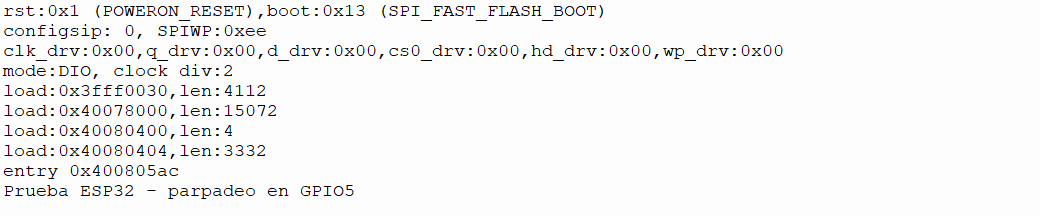
\includegraphics[width=0.7\textwidth]{MicroPython/test.png}
  \caption{Salida del programa de prueba en la consola de Thonny.}
\end{figure}

\section{Resultados}

En esta sección se muestran las evidencias experimentales obtenidas tras la carga y ejecución de los programas desarrollados en el ESP32 mediante Thonny.  
Cada fotografía corresponde al funcionamiento real de los circuitos descritos en las prácticas.

\subsection{Parpadeo del LED en GPIO5}
El LED conectado al pin GPIO5 alterna su estado cada segundo, evidenciando el correcto funcionamiento del programa \texttt{blink\_pin5.py} y la configuración del pin como salida digital.

\begin{figure}[H]
  \centering
  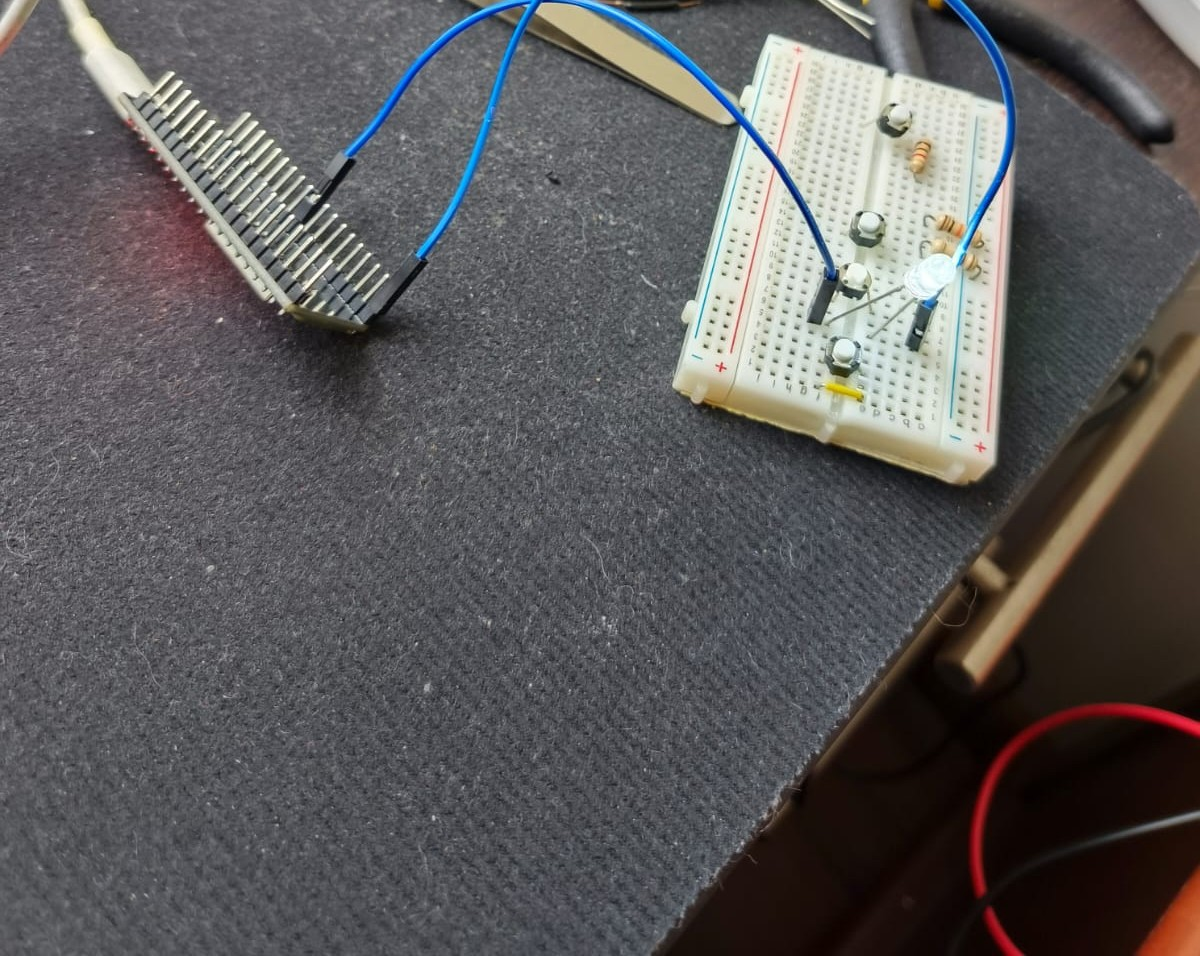
\includegraphics[width=0.65\textwidth]{Resultados/LED.jpg}
  \caption{LED conectado al GPIO5 parpadeando con un periodo aproximado de 1\,s.}
\end{figure}

\subsection{Control de LED mediante pulsador en GPIO16}
En la segunda prueba, el pulsador conectado al pin GPIO16 controla el encendido del LED.  
El uso del resistor de \texttt{pull-up} interno y el manejo de rebote por software permiten una respuesta estable sin parpadeos erráticos.

\begin{figure}[H]
  \centering
  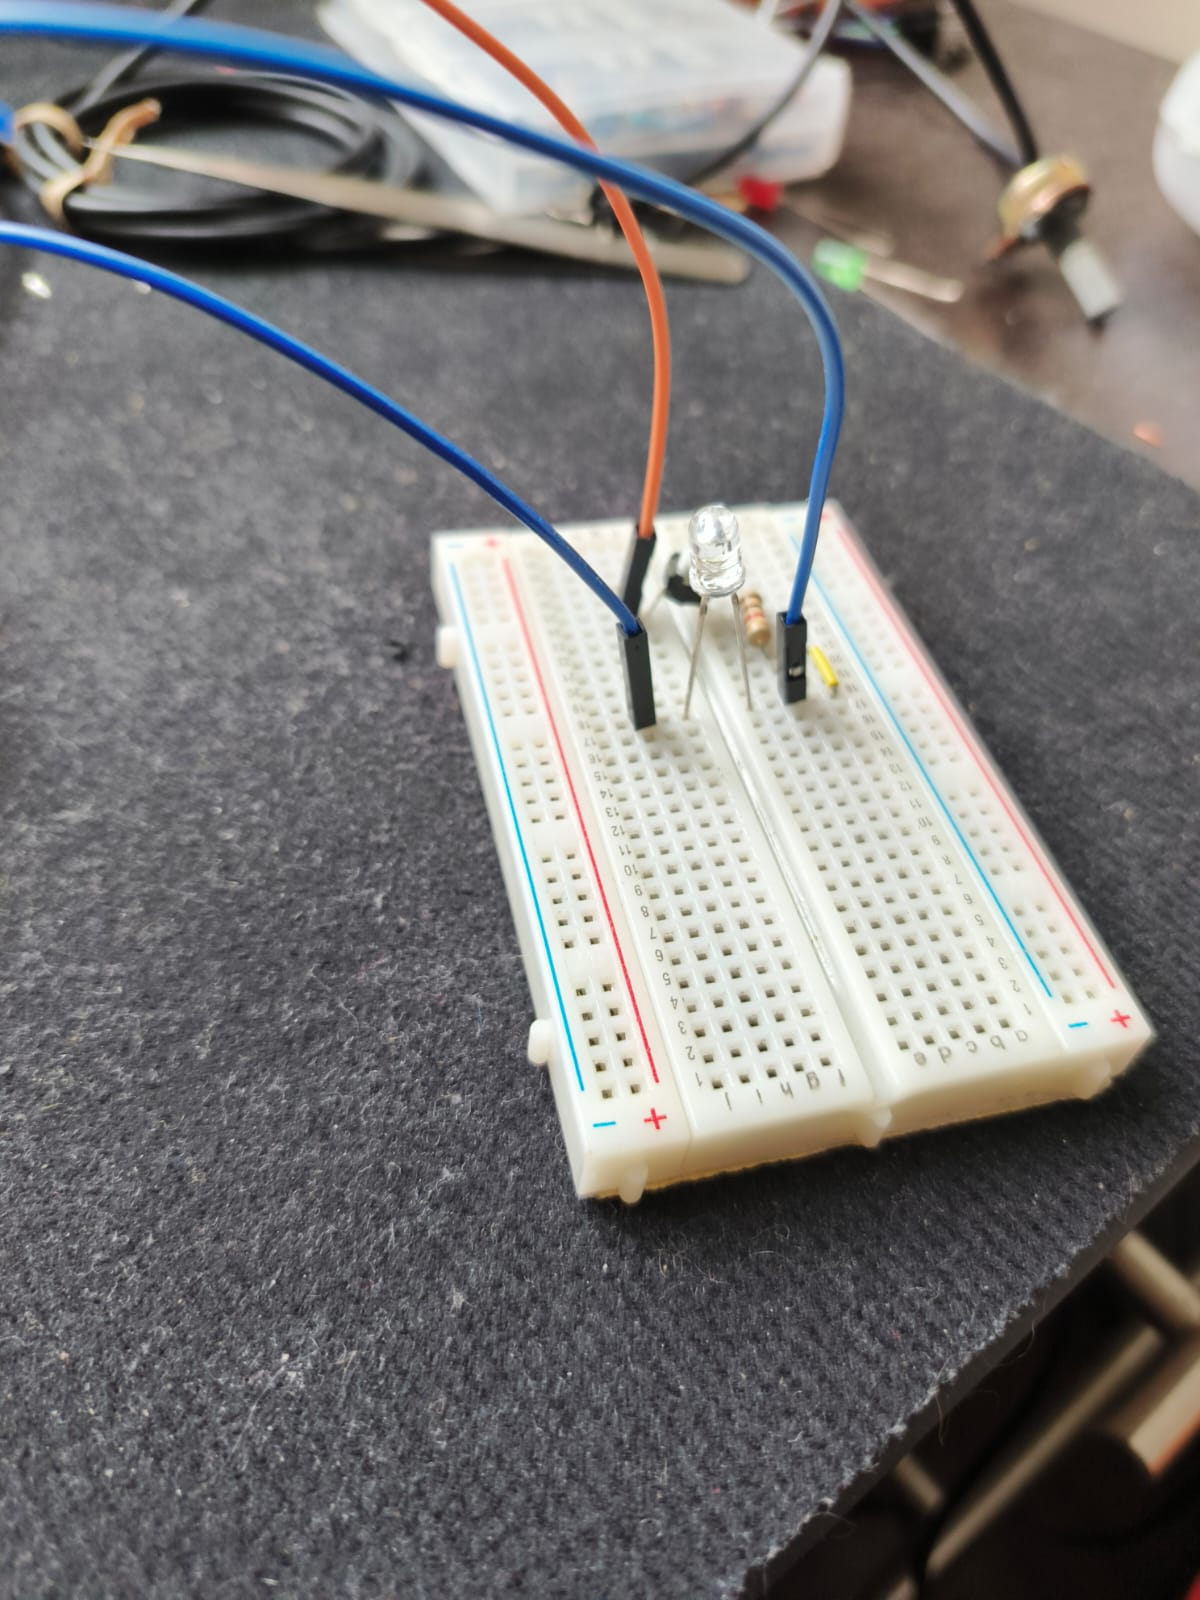
\includegraphics[width=0.55\textwidth]{Resultados/pULSANTE.jpg}
  \caption{LED controlado por un pulsador (GPIO16), activo al presionar.}
\end{figure}

\begin{figure}[H]
  \centering
  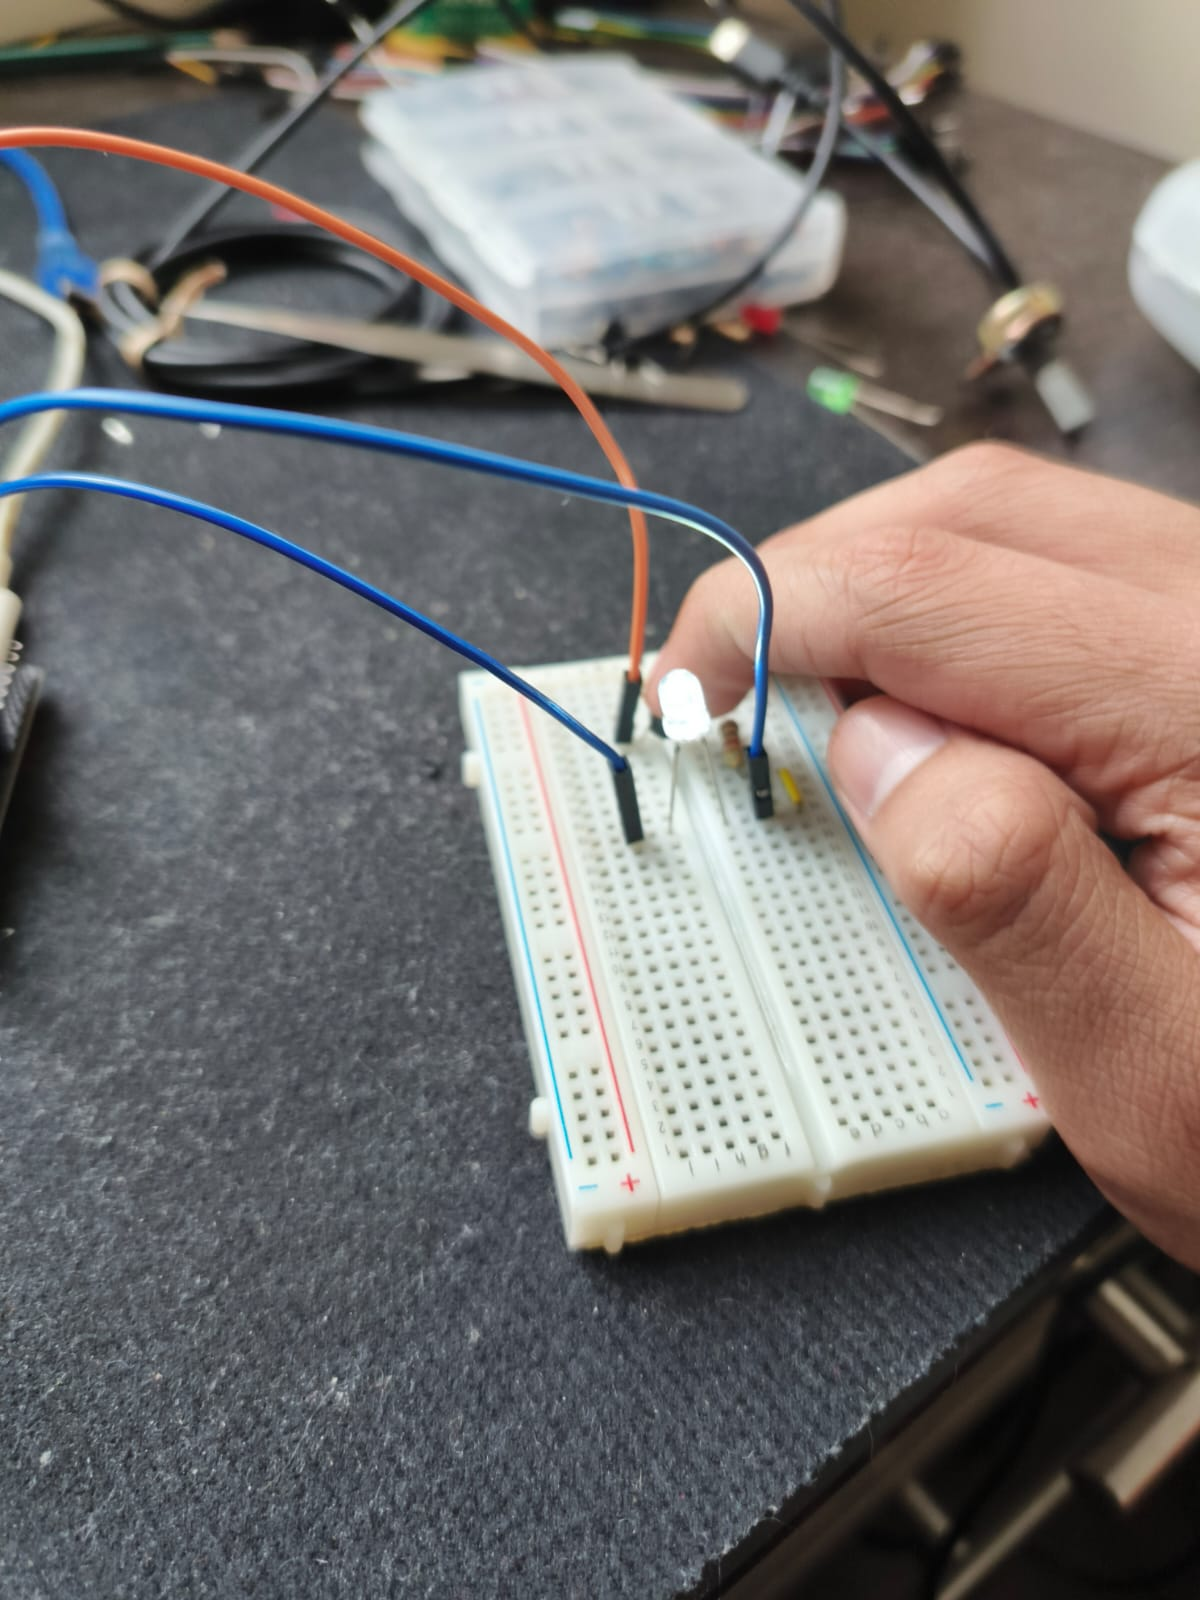
\includegraphics[width=0.45\textwidth]{Resultados/PULSANTE_1.jpg}
  \caption{LED controlado por un pulsador (GPIO16), activo al presionar.}
\end{figure}

\subsection{Lectura analógica del potenciómetro en GPIO34}
Finalmente, el programa \texttt{adc\_pot\_esp32.py} permite visualizar las lecturas del ADC en la consola de Thonny, mostrando valores proporcionales a la posición del potenciómetro.

\begin{figure}[H]
  \centering
  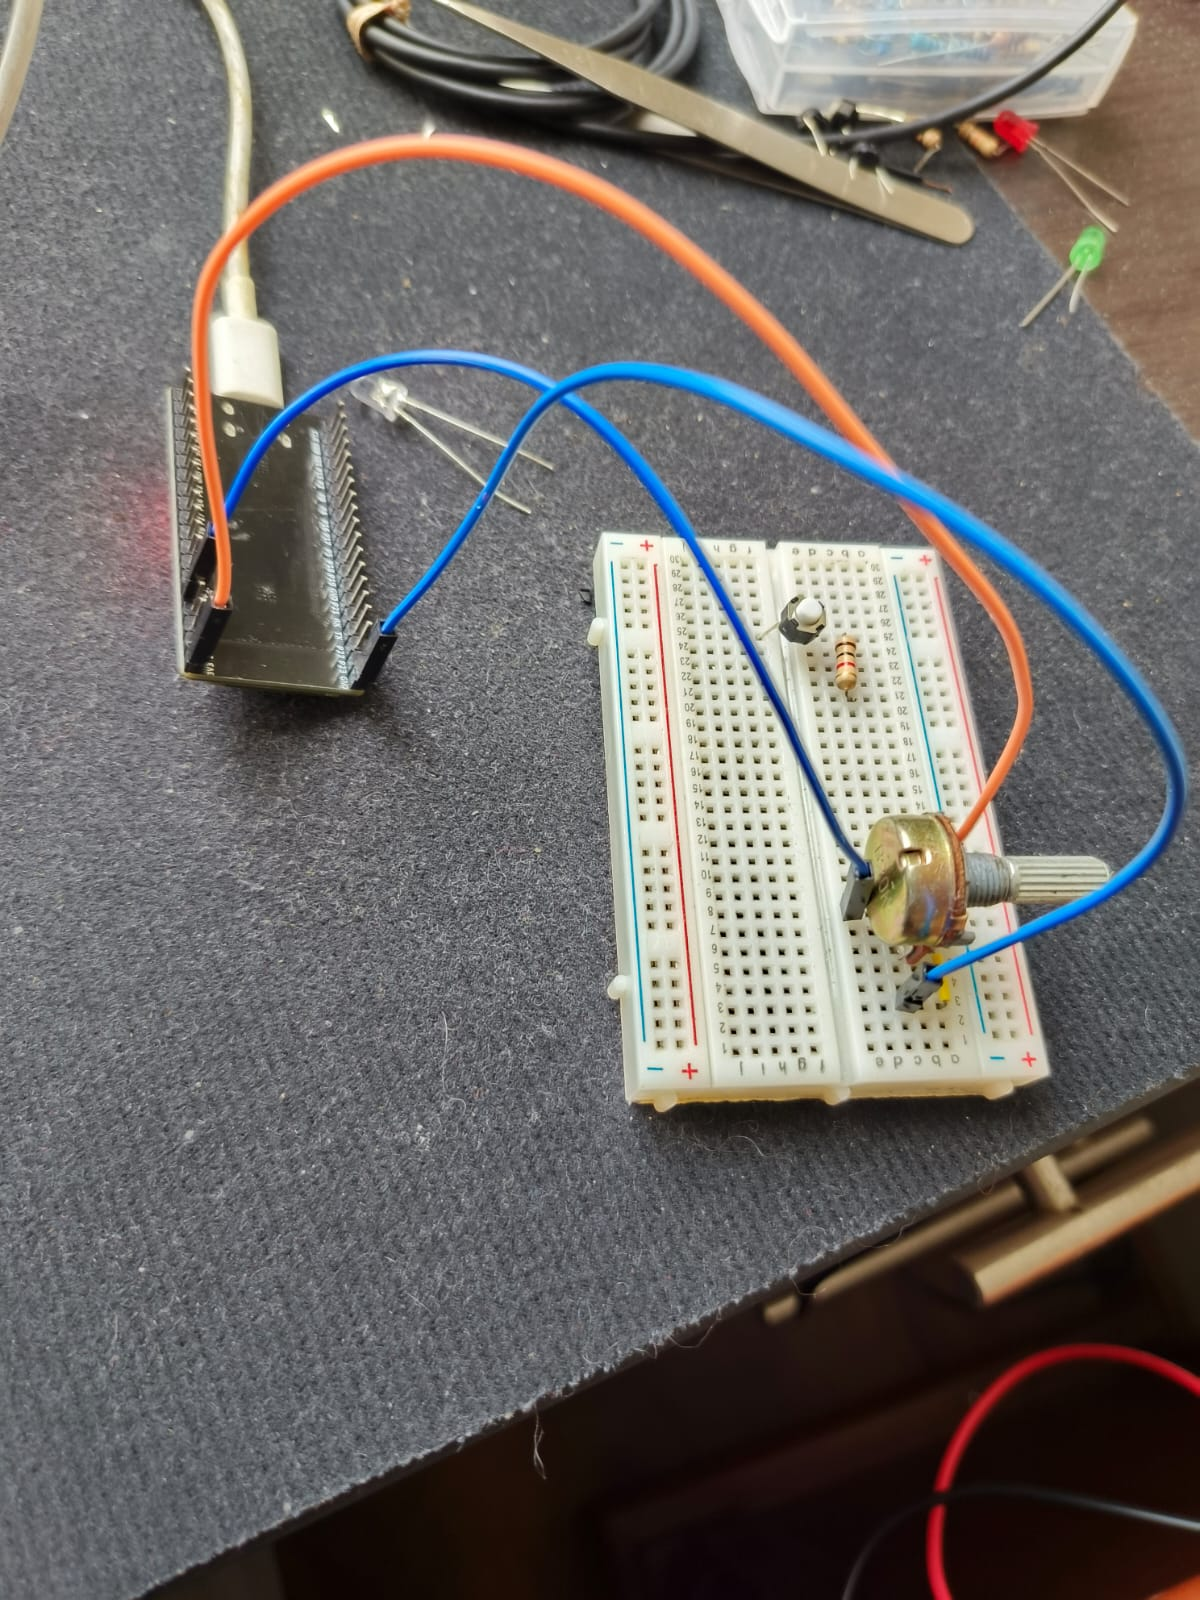
\includegraphics[width=0.45\textwidth]{Resultados/POTENCIOMETRO.jpg}
  \caption{Lectura analógica de un potenciómetro en GPIO34 con salida en la consola.}
\end{figure}

\begin{figure}[H]
  \centering
  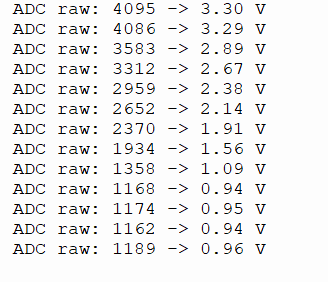
\includegraphics[width=0.65\textwidth]{Resultados/ADC.png}
  \caption{Lectura analógica de un potenciómetro en GPIO34 con salida en la consola.}
\end{figure}






\end{document}
